\documentclass[11pt,a4paper]{article}

% ═══ Packages ═══
\usepackage[margin=2cm]{geometry}
\usepackage{kotex}
\usepackage{enumitem}
\usepackage{titlesec}
\usepackage{xcolor}
\usepackage{hyperref}
\usepackage{fancyhdr}
\usepackage{tabularx}
\usepackage{fontawesome5}
\usepackage{graphicx}
\usepackage{wrapfig}

% ═══ Colors ═══
\definecolor{accent}{HTML}{2856A0}
\definecolor{darktext}{HTML}{1a2332}
\definecolor{lighttext}{HTML}{5a6578}

% ═══ Hyperref ═══
\hypersetup{
  colorlinks=true,
  linkcolor=accent,
  urlcolor=accent,
  pdfauthor={Jungseob Lee},
  pdftitle={General CV - Jungseob Lee},
}

% ═══ Formatting ═══
\pagestyle{fancy}
\fancyhf{}
\renewcommand{\headrulewidth}{0pt}
\fancyfoot[C]{\footnotesize\color{lighttext} Jungseob Lee --- Curriculum Vitae --- \thepage}

\titleformat{\section}{\large\bfseries\color{accent}}{}{0em}{}[\titlerule]
\titlespacing*{\section}{0pt}{16pt}{8pt}

\titleformat{\subsection}{\bfseries\color{darktext}}{}{0em}{}
\titlespacing*{\subsection}{0pt}{9pt}{3pt}

\setlength{\parindent}{0pt}
\setlist[itemize]{leftmargin=1.5em, itemsep=2pt, parsep=0pt}

% ═══ Commands ═══
\newcommand{\cventry}[4]{%
  \textbf{#1} \hfill \textit{#2} \\
  \textit{#3} \hfill #4 \vspace{4pt}\\
}
\newcommand{\me}[1]{\textbf{\underline{#1}}}
\newcommand{\papertitle}[1]{\textit{``#1''}}
\newcommand{\paperlink}[1]{\href{#1}{[\textcolor{accent}{PDF}]}}
\newcommand{\doilink}[1]{\href{#1}{[\textcolor{accent}{DOI}]}}
\newcommand{\arxivlink}[1]{\href{#1}{[\textcolor{accent}{arXiv}]}}
\newcommand{\codelink}[1]{\href{#1}{[\textcolor{accent}{Code}]}}

\begin{document}

% ═══════════════════════════════════════════
%  Header
% ═══════════════════════════════════════════
\begin{minipage}[c]{0.22\textwidth}
  \centering
  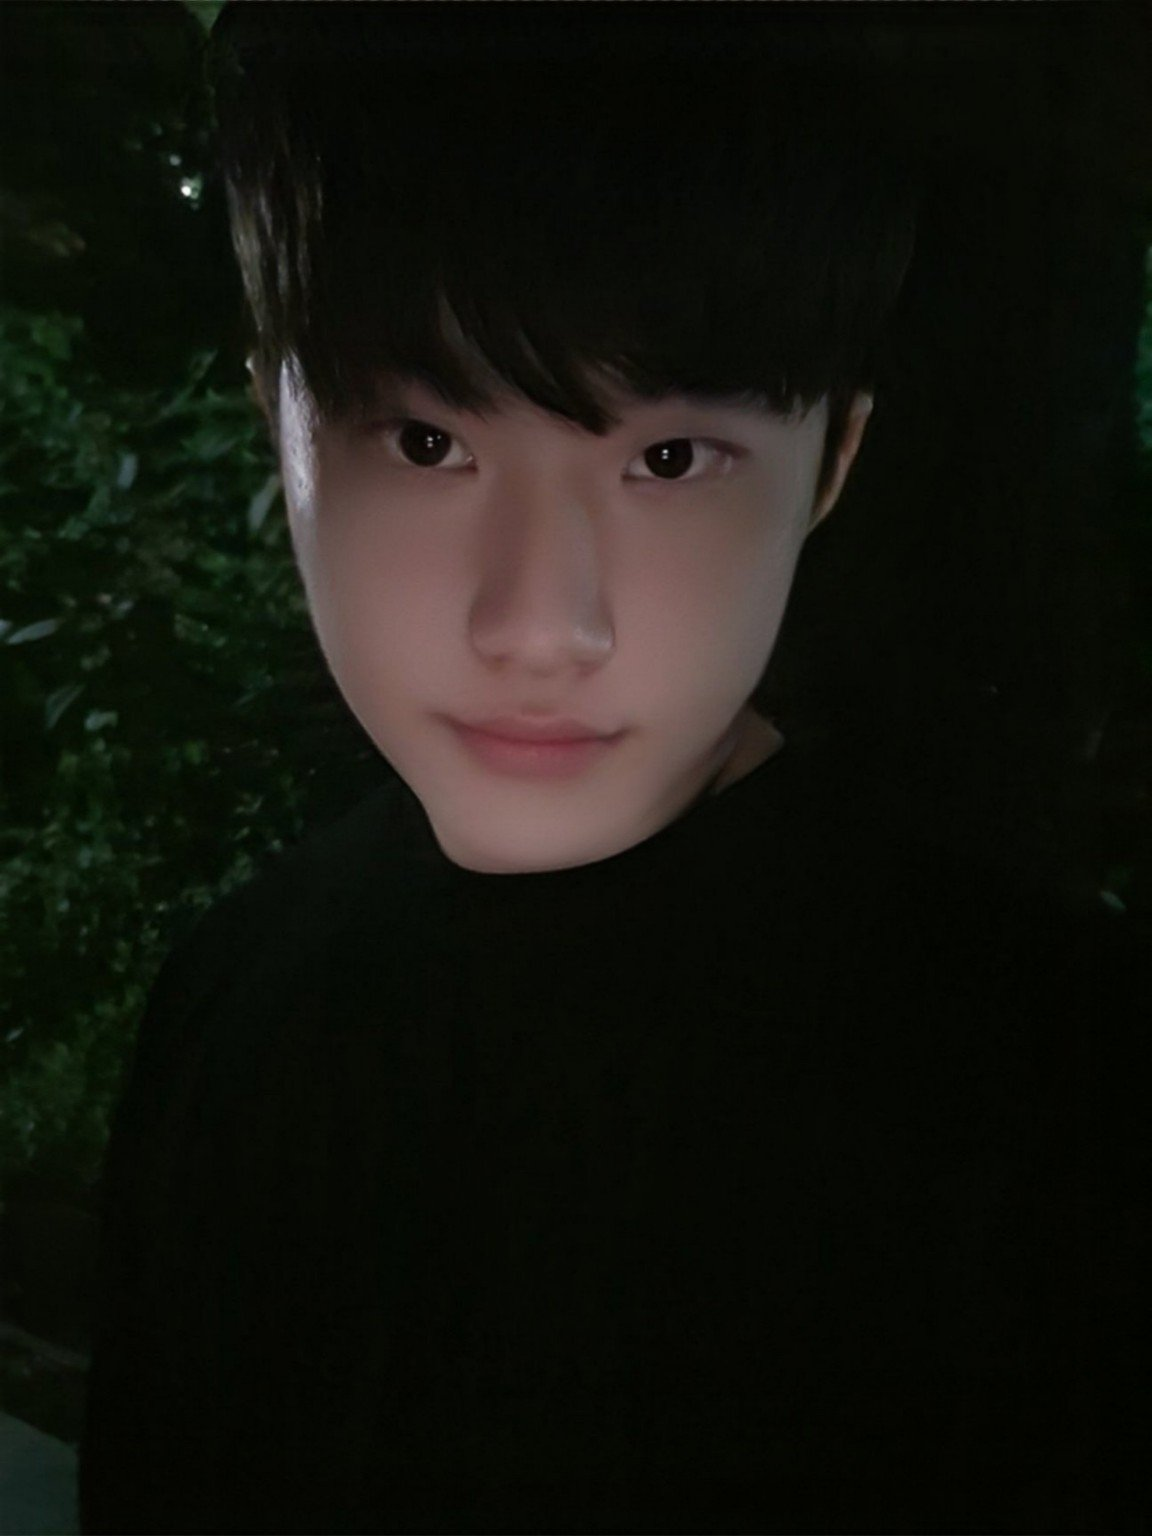
\includegraphics[width=3.2cm]{photo.jpg}
\end{minipage}%
\hfill
\begin{minipage}[c]{0.75\textwidth}
  \begin{center}
    {\LARGE\bfseries Jungseob Lee} \\[6pt]
    {\color{lighttext} NLP Researcher $\cdot$ Graduate Student, Korea University} \\[10pt]
    \begin{tabular}{ccc}
      \faIcon{birthday-cake}~1995.10.11 &
      \faIcon{envelope}~\href{mailto:omanma1928@korea.ac.kr}{omanma1928@korea.ac.kr} &
      \faIcon{globe}~\href{https://js-lee-ai.github.io}{js-lee-ai.github.io} \\[3pt]
      \faIcon{github}~\href{https://github.com/js-lee-AI}{js-lee-AI} &
      \faIcon{linkedin}~\href{https://www.linkedin.com/in/jslee-nlp/}{LinkedIn} &
      \faIcon{graduation-cap}~\href{https://scholar.google.com/citations?hl=ko&user=dTBGyFIAAAAJ}{Google Scholar}
    \end{tabular}
  \end{center}
\end{minipage}

\vspace{4pt}

% ═══════════════════════════════════════════
%  Summary
% ═══════════════════════════════════════════
\section{Summary}
Integrated M.S./Ph.D. researcher at the Korea University NLP Lab (Advisor: Prof.~Heuiseok Lim), specializing in large language models and natural language processing --- with a focus on agentic LLMs, efficient reasoning, machine translation, information retrieval, and model merging. First-author research has been published at \textbf{EMNLP 2026} (Main), \textbf{ACL 2025} (Oral), and \textbf{Findings of ACL 2024}. Four papers were accepted at \textbf{EMNLP 2026} (2 Main, 2 Findings), with co-authored work at \textbf{ICLR 2026} and a series of preprints under review. Recipient of the \textbf{Best Paper Award (Top~1)} at HCLT 2025. Served as the post-training Project Manager and Korea University representative for \textbf{VAETKI}, Korea's national Sovereign AI Foundation Model. Author of 30+ peer-reviewed papers across top-tier NLP venues and journals.

% ═══════════════════════════════════════════
%  Education
% ═══════════════════════════════════════════
\section{Education}
\cventry{Integrated M.S./Ph.D. in Computer Science}{2021 -- Present}{Korea University, Seoul, Korea}{\textbf{Expected: Feb. 2027}}
\begin{itemize}
  \item NLP Lab, Advisor: Prof.~Heuiseok Lim.
  \item Research focus: large language models, natural language processing, agentic LLM, efficient reasoning, machine translation, information retrieval, and model merging.
\end{itemize}

% ═══════════════════════════════════════════
%  Research Interests
% ═══════════════════════════════════════════
\section{Research Interests}
Large Language Models $\cdot$ Natural Language Processing $\cdot$ Agentic LLM $\cdot$ Efficient Reasoning $\cdot$ Machine Translation $\cdot$ Information Retrieval $\cdot$ Model Merging

% ═══════════════════════════════════════════
%  Work Experience & Major Projects
% ═══════════════════════════════════════════
\section{Work Experience \& Major Projects}

\textbf{VAETKI --- Korean Sovereign AI Foundation Model} \hfill \textit{Jun 2025 -- Jan 2026} \\
\textit{Post-training Project Manager --- Korea University Representative} \hfill {\footnotesize\color{lighttext} NC AI (NCSOFT)-led consortium} \\[2pt]
\begin{itemize}
  \item Served as post-training PM representing Korea University in Korea's national \textbf{Sovereign AI Foundation Model} program, organized by the Ministry of Science and ICT --- an approximately KRW~200~billion national initiative with staged six-month evaluations running through 2027.
  \item The Korea University team (Prof.~Heuiseok Lim) was selected as a core research partner in the NC~AI (NCSOFT)-led grand consortium of 14 industry--academia--research institutions and 40 adopters (including POSCO~DX, Lotte Innovate, KAIST, ETRI, and MBC).
  \item Led the full post-training pipeline --- Supervised Fine-Tuning (SFT), Reinforcement Learning, and dataset curation --- for the VAETKI model.
  \item \textbf{VAETKI model:} an industry-specialized sovereign foundation model, open-sourced on Hugging Face on Dec~30, 2025. A 100B+ parameter Mixture-of-Experts architecture (~11B active parameters at inference) with a custom Multi-head Latent Attention (MLA) reducing memory usage by up to ~83\%.
  \item Achieved state-of-the-art results on Korean language and culture (CLIcK), advanced reasoning (KoBALT), professional knowledge (KMMLU-Pro), and instruction following (IFEval).
  \item \href{https://huggingface.co/NC-AI-consortium-VAETKI/VAETKI}{[\textcolor{accent}{Model}]} \enspace \href{https://github.com/wbl-ncai/VAETKI/blob/releases/v1.0.0/VAETKI_Technical_Report.pdf}{[\textcolor{accent}{Technical Report}]}
  \item Press: \href{https://www.korea.ac.kr/bbs/ko/42/120917/artclView.do}{[\textcolor{accent}{Korea University}]} \enspace \href{https://www.yna.co.kr/view/RPR20230926008900353}{[\textcolor{accent}{Yonhap News}]} \enspace \href{https://www.aitimes.kr/news/articleView.html?idxno=37944}{[\textcolor{accent}{AI Times}]} \enspace \href{https://www.newstomato.com/ReadNews.aspx?no=1270232}{[\textcolor{accent}{Newstomato}]}
\end{itemize}
\vspace{5pt}

\textbf{Cross-lingual Language Transfer for Large Language Models} \hfill \textit{2024 -- 2025} \\
\textit{Lead Researcher (first author)} \hfill {\footnotesize\color{lighttext} Published at ACL 2025 (Oral)} \\[2pt]
\begin{itemize}
  \item Proposed a cross-lingual optimization method that efficiently transfers English-centric LLMs to new target languages while preserving source-language ability; accepted as an \textbf{Oral} presentation at ACL 2025.
  \item \href{https://aclanthology.org/2025.acl-long.734.pdf}{[\textcolor{accent}{PDF}]}
\end{itemize}
\vspace{5pt}

\textbf{Efficient Reasoning for Large Reasoning Models} \hfill \textit{2025 -- Present} \\
\textit{Lead Researcher (first author)} \hfill {\footnotesize\color{lighttext} Findings of EMNLP 2026; preprints under review} \\[2pt]
\begin{itemize}
  \item Leading a first-author line of work on training-free adaptive thinking budgets (DART) and stable efficiency training via adaptive correct-only rewards (ACOER) for large reasoning models; DART was accepted to \textbf{Findings of EMNLP 2026}.
  \item Co-first author of \textbf{ThinkFuse}, a trajectory-aware test-time fusion method for small reasoning models, accepted to \textbf{Findings of EMNLP 2026}.
  \item \href{https://arxiv.org/abs/2606.23181}{[\textcolor{accent}{DART}]} \enspace \href{https://arxiv.org/abs/2606.22716}{[\textcolor{accent}{ACOER}]} \enspace \href{https://github.com/js-lee-AI/DART}{[\textcolor{accent}{Code}]}
\end{itemize}

% ═══════════════════════════════════════════
%  Awards
% ═══════════════════════════════════════════
\section{Awards}
\textbf{Best Paper Award (Top 1)} \hfill \textit{2025} \\
Annual Conference on Human and Cognitive Language Technology (HCLT 2025) \\[2pt]
{\small For \papertitle{KULLM-RAG: A RAG-Specialized Large Language Model with Intelligent Self-Verification}; \me{J.~Lee} (first author), M.~Kim, J.~Yoon, S.~Hong, Y.~Jang, S.~Lee, J.~Seo, C.~Park, J.~Park, H.~Lim --- Korea University; Soongsil University; Human-Inspired AI Research.}

% ═══════════════════════════════════════════
%  Publications
% ═══════════════════════════════════════════
\section{Publications}
{\small\color{lighttext} \underline{Underlined} = author. $^{*}$ denotes equal contribution. Full profile on \href{https://scholar.google.com/citations?hl=ko&user=dTBGyFIAAAAJ}{\textcolor{accent}{Google Scholar}}.}
\vspace{4pt}

{\small

\subsection*{2026}
\begin{itemize}
  \item \papertitle{The Geometry of Hallucination Detection: Why Simple Probes Are Sufficient} \\
    \me{J.~Lee}, J.~Seo, H.~Lim \enspace---\enspace \textbf{EMNLP 2026} (Main)

  \item \papertitle{Language Chain in Alignment: Cross-Lingual Ranking Preference Optimization} \\
    S.~Lee, M.~Kim, \me{J.~Lee}, H.~Lim \enspace---\enspace \textbf{EMNLP 2026} (Main)

  \item \papertitle{DART: Draft-Agreement Routing for Training-Free Adaptive Thinking Budgets in Hybrid Reasoning Models} \\
    \me{J.~Lee}, S.~Hong, S.~Lee, J.~Seo, J.~Son, S.~Eo, C.~Park, H.~Park, H.~Moon, H.~Lim \enspace---\enspace \textbf{Findings of EMNLP 2026} \enspace \arxivlink{https://arxiv.org/abs/2606.23181} \enspace \codelink{https://github.com/js-lee-AI/DART}

  \item \papertitle{ThinkFuse: Trajectory-Aware Test-Time Fusion for Small Reasoning Models} \\
    M.~Kang$^{*}$, \me{J.~Lee}$^{*}$, J.~Seo, H.~Lim \enspace---\enspace \textbf{Findings of EMNLP 2026} ($^{*}$equal contribution)

  \item \papertitle{Improving Semantic Proximity in Information Retrieval through Cross-Lingual Alignment} \\
    S.~Hong, Y.~Jang, \me{J.~Lee}, H.~Moon, H.~Lim \enspace---\enspace \textbf{ICLR 2026} (Poster) \enspace \paperlink{https://openreview.net/pdf?id=NvKvW5k6Kk}

  \item \papertitle{Towards Enhancing Natural Language Inference for Identifying Erroneous Outputs in Data-to-Text Generation} \\
    C.~Ok, E.K.~Lee, H.~Ju, \me{J.~Lee}, D.~Oh \enspace---\enspace \textbf{Knowledge-Based Systems} \enspace \doilink{https://www.sciencedirect.com/science/article/pii/S0950705126006878}

  \item \papertitle{Beyond Penalizing Mistakes: Stabilizing Efficiency Training in Large Reasoning Models via Adaptive Correct-Only Rewards} \\
    \me{J.~Lee}, S.~Lee, S.~Hong, M.~Kim, C.~Park, H.~Lim \enspace---\enspace Preprint, under review \enspace \arxivlink{https://arxiv.org/abs/2606.22716} \enspace \codelink{https://github.com/js-lee-AI/ACOER}

  \item \papertitle{To Isolate or to Score? Model-Adaptive Assessment for Cost-Efficient Multi-Agent RAG} \\
    \me{J.~Lee}, C.~Park, H.~Lim \enspace---\enspace Preprint, under review \enspace \arxivlink{https://arxiv.org/abs/2606.25191} \enspace \codelink{https://github.com/js-lee-AI/MADARA}

  \item \papertitle{Skin-Deep: A Geometric Diagnostic for Alignment Fragility in Large Language Model Representations} \\
    D.J.~Lee$^{*}$, \me{J.~Lee}$^{*}$, S.~Lee, S.~Hong, S.~Son, S.~Eo, J.~Seo, H.~Lim \enspace---\enspace Preprint, under review ($^{*}$equal contribution) \enspace \arxivlink{https://arxiv.org/abs/2606.22676} \enspace \codelink{https://github.com/js-lee-AI/skin-deep}
\end{itemize}

\subsection*{2025}
\begin{itemize}
  \item \papertitle{Cross-lingual Optimization for Language Transfer in Large Language Models} \\
    \me{J.~Lee}, S.~Hong, H.~Moon, H.S.~Lim \enspace---\enspace \textbf{ACL 2025} (Oral) \enspace \paperlink{https://aclanthology.org/2025.acl-long.734.pdf}

  \item \papertitle{KULLM-RAG: A RAG-Specialized Large Language Model with Intelligent Self-Verification} \\
    \me{J.~Lee}, M.~Kim, J.~Yoon, S.~Hong, Y.~Jang, S.~Lee, J.~Seo, C.~Park, J.~Park, H.~Lim \enspace---\enspace Annual Conference on Human and Cognitive Language Technology (HCLT 2025) --- \textbf{Best Paper Award}

  \item \papertitle{An Analysis on Language Transfer of Pre-trained Language Model with Cross-lingual Post-training} \\
    S.~Son, C.~Park, \me{J.~Lee}, M.~Shim, C.~Lee, Y.~Jang, J.~Seo, J.~Lim, H.~Lim \enspace---\enspace \textbf{Expert Systems with Applications} \enspace \doilink{https://doi.org/10.1016/j.eswa.2024.125841}

  \item \papertitle{VAETKI Technical Report} \\
    NC~AI Consortium \enspace---\enspace Technical Report \enspace \paperlink{https://github.com/wbl-ncai/VAETKI/blob/releases/v1.0.0/VAETKI_Technical_Report.pdf}
\end{itemize}

\subsection*{2024}
\begin{itemize}
  \item \papertitle{Length-aware Byte Pair Encoding for Mitigating Over-segmentation in Korean Machine Translation} \\
    \me{J.~Lee}, H.~Moon, S.~Lee, C.~Park, S.~Eo, H.~Ko, J.~Seo, S.~Lee, H.S.~Lim \enspace---\enspace \textbf{Findings of ACL 2024} \enspace \paperlink{https://aclanthology.org/2024.findings-acl.135.pdf}

  \item \papertitle{Analysis of the Effectiveness of Model, Data, and User-Centric Approaches for Chat Application: A Case Study of BlenderBot 2.0} \\
    C.~Park, \me{J.~Lee}, S.~Son, K.~Park, J.~Jang, H.~Lim \enspace---\enspace \textbf{Applied Sciences} \enspace \doilink{https://doi.org/10.3390/app14114821}
\end{itemize}

\subsection*{2023}
\begin{itemize}
  \item \papertitle{PEEP-Talk: A Situational Dialogue-based Chatbot for English Education} \\
    S.~Lee, Y.~Jang, C.~Park, \me{J.~Lee}, J.~Seo, H.~Moon, S.~Eo, S.~Lee, B.~Yahya, \textit{et al.} \enspace---\enspace \textbf{ACL 2023} (System Demonstrations) \enspace \paperlink{https://aclanthology.org/2023.acl-demo.18.pdf}

  \item \papertitle{A Survey on Evaluation Metrics for Machine Translation} \\
    S.~Lee, \me{J.~Lee}, H.~Moon, C.~Park, J.~Seo, S.~Eo, S.~Koo, H.~Lim \enspace---\enspace \textbf{Mathematics} \enspace \paperlink{https://www.mdpi.com/2227-7390/11/4/1006}

  \item \papertitle{Doubts on the Reliability of Parallel Corpus Filtering} \\
    H.~Moon, C.~Park, S.~Koo, \me{J.~Lee}, S.~Lee, J.~Seo, S.~Eo, Y.~Jang, H.~Kim, H.~Lee, \textit{et al.} \enspace---\enspace \textbf{Expert Systems with Applications} \enspace \doilink{https://doi.org/10.1016/j.eswa.2023.120962}

  \item \papertitle{KoCheckGPT: Korean LLM Written Document Detector} \\
    M.~Kang, \me{J.~Lee}, S.~Lee, S.~Hong, J.~Park, H.~Lim \enspace---\enspace Annual Conference on Human and Language Technology (HCLT 2023) \enspace \paperlink{https://koreascience.kr/article/CFKO202306643317050.page}
\end{itemize}

\subsection*{2022}
\begin{itemize}
  \item \papertitle{QUAK: A Synthetic Quality Estimation Dataset for Korean-English Neural Machine Translation} \\
    S.~Eo, C.~Park, H.~Moon, J.~Seo, G.~Kim, \me{J.~Lee}, H.S.~Lim \enspace---\enspace \textbf{COLING 2022} \enspace \paperlink{https://aclanthology.org/2022.coling-1.460.pdf}

  \item \papertitle{Empirical Analysis of Noising Scheme based Synthetic Data Generation for Automatic Post-editing} \\
    H.~Moon, C.~Park, S.~Lee, J.~Seo, \me{J.~Lee}, S.~Eo, H.S.~Lim \enspace---\enspace \textbf{LREC 2022} \enspace \paperlink{https://aclanthology.org/2022.lrec-1.93.pdf}

  \item \papertitle{K-NCT: Korean Neural Grammatical Error Correction Gold-standard Test Set Using Novel Error Type Classification Criteria} \\
    S.~Koo, C.~Park, J.~Seo, S.~Lee, H.~Moon, \me{J.~Lee}, H.~Lim \enspace---\enspace \textbf{IEEE Access} \enspace \paperlink{https://ieeexplore.ieee.org/document/9938990}

  \item \papertitle{Focus on FoCus: Is FoCus Focused on Context, Knowledge and Persona?} \\
    S.Y.~Lee, \me{J.~Lee}, C.~Park, S.~Eo, H.~Moon, J.~Seo, J.~Park, H.S.~Lim \enspace---\enspace 1st Workshop on Customized Chat Grounding Persona and Knowledge \enspace \paperlink{https://aclanthology.org/2022.ccgpk-1.1.pdf}

  \item \papertitle{There is No Rose Without a Thorn: Finding Weaknesses on BlenderBot 2.0} \\
    \me{J.~Lee}, M.~Shim, S.~Son, C.~Park, Y.~Kim, H.~Lim \enspace---\enspace arXiv preprint \enspace \arxivlink{https://arxiv.org/pdf/2201.03239}

  \item \papertitle{Language Chameleon: Transformation Analysis between Languages Using Cross-lingual Post-training} \\
    S.~Son, C.~Park, \me{J.~Lee}, M.~Shim, C.~Lee, Y.~Jang, J.~Seo, H.~Lim \enspace---\enspace arXiv preprint \enspace \arxivlink{https://arxiv.org/abs/2209.06422}

  \item \papertitle{Korean and Multilingual Language Models Study for Cross-lingual Post-training (XPT)} \\
    S.~Son, C.~Park, \me{J.~Lee}, M.~Shim, C.~Lee, K.~Park, H.~Lim \enspace---\enspace \textbf{Journal of the Korea Convergence Society} \enspace \paperlink{https://koreascience.kr/article/JAKO202210459401088.page}

  \item \papertitle{Policy-based Performance Comparison Study of Real-time Simultaneous Translation} \\
    \me{J.~Lee}, H.~Moon, C.~Park, J.~Seo, S.~Eo, S.~Lee, S.~Koo, H.~Lim \enspace---\enspace \textbf{Journal of the Korea Convergence Society} \enspace \paperlink{https://www.koreascience.kr/article/JAKO202210459432095.page}

  \item \papertitle{SaJuTeller: Conditional Generation Deep-Learning based Fortune Telling Model} \\
    H.~Moon, \me{J.~Lee}, J.~Seo, S.~Eo, C.~Park, W.~Kim, J.~Park, H.~Lim \enspace---\enspace Annual Conference on Human and Language Technology (HCLT 2022) \enspace \paperlink{https://koreascience.kr/article/CFKO202226455345621.view}

  \item \papertitle{Korean Language Model Construction and Comparative Analysis with Cross-lingual Post-Training (XPT)} \\
    S.~Son, C.~Park, \me{J.~Lee}, M.~Shim, S.~Lee, J.W.~Lee, A.~So, H.~Lim \enspace---\enspace Annual Conference on Human and Language Technology (HCLT 2022) \enspace \paperlink{https://koreascience.kr/article/CFKO202226455345799.page}

  \item \papertitle{DART: Data Augmentation using Retrieval Technique} \\
    S.~Lee, J.~Seo, \me{J.~Lee}, M.~Kang, H.~Moon, C.~Park, D.~Jung, J.~Lee, K.~Park, \textit{et al.} \enspace---\enspace Annual Conference on Human and Language Technology (HCLT 2022) \enspace \paperlink{https://www.koreascience.kr/article/CFKO202226455346012.page}
\end{itemize}

\subsection*{2021}
\begin{itemize}
  \item \papertitle{Empirical Study on BlenderBot 2.0's Errors Analysis in Terms of Model, Data and Dialogue} \\
    \me{J.~Lee}, S.~Son, M.~Shim, Y.~Kim, C.~Park, A.~So, J.~Park, H.~Lim \enspace---\enspace \textbf{Journal of the Korea Convergence Society} \enspace \paperlink{https://www.koreascience.or.kr/article/JAKO202106361939222.page}
\end{itemize}

}

\vfill
\begin{center}
  \color{lighttext}\footnotesize Last updated: \today
\end{center}

\end{document}
